%\mag 1200
%\mag 1150
%\mag 1250
%\mag 1071
\documentclass[12pt, openany, oneside]{book} % Computer Modern font calls
\usepackage[paper=a4paper]{geometry}
%\usepackage[paper=a4paper, twoside]{geometry}

\usepackage[T2A]{fontenc}
%\usepackage{literat}
%\usepackage[pdftex,unicode]{hyperref}
\usepackage[dvips]{graphicx}
\usepackage{longtable}
\usepackage[utf8]{inputenc}
\usepackage[english,russian]{babel}
\usepackage[14pt]{extsizes}
\usepackage{fancyhdr}
\usepackage{pstricks}
\usepackage{pst-all}
\usepackage{pst-poly}
\usepackage{indentfirst}
\usepackage{pscyr}
\usepackage{blindtext}

%\usepackage{times}
%\usepackage{pslatex}
%\def\defgeom{\geometry{paper=a5paper, left=1.4142cm, top=1.4142cm, bottom=1.4142cm,
%centering, right=1.4142cm, bindingoffset=0mm, }}
%\def\defgeom{\geometry{papersize={17.5cm,24.75cm}, left=2.25cm, right=2.25cm, top=1.5cm, bottom=2.33cm, centering, bindingoffset=1mm}}
%\def\defgeom{\geometry{papersize={21cm,29.7cm}, left=2.7cm, right=2.7cm, top=1.8cm, bottom=2.8cm, centering, bindingoffset=1mm}}
%\def\defgeom{\geometry{paper=a4paper, left=2.7cm, right=2.7cm, top=1.8cm, bottom=2.8cm, centering, bindingoffset=1mm}}
\def\defgeom{\geometry{paper=a4paper, left=2.7cm, top=1.8cm, bottom=2.8cm, centering, right=2.7cm, bindingoffset=1mm}}
\tolerance=10000

%Основные требования для макетов в редакторе Тех
%Поля: верхнее – 1,8 см, нижнее – 2,8, левое и правое – 2,7
%Расстояние от края страницы до колонтитула – 2,1 см

%\def\normalsize{\fontsize{15}{18}\selectfont{}}

\newenvironment{PP}{%
    \begin{quote}\tt}{%
    \end{quote}}
\def\rem#1{}


 %\renewcommand{\publishername}{Иркутский государственный технический университет}
 %\renewcommand{\locationname}{Иркутск}
%\def\AR{{\em Прим.~автора~пособия}}
 \def\baselinestretch{1}

\newtheorem{example}{Пример}[chapter]
\newenvironment{mygroup}{}{}

 \setcounter{secnumdepth}{3}
 \setcounter{tocdepth}{3}

%\defgeom{}
\makeatletter
\def\@makechapterhead#1{%
  %\vspace*{10\p@}%
  {\parindent \z@ \raggedright \normalfont
    \ifnum \c@secnumdepth >\m@ne
      \if@mainmatter
        \large\bfseries \@chapapp\space \thechapter. \hbox to 0.3em {}
        %\par\nobreak
        %\vskip 5\p@
      \fi
    \fi
    \interlinepenalty\@M
    % \Large \bfseries #1\par\nobreak
    \large \bfseries #1\par\nobreak
    \vskip 7\p@
  }}
\def\@makeschapterhead#1{%
  %\vspace*{50\p@}%
  {\parindent \z@ \raggedright
    \normalfont
    \interlinepenalty\@M
    \large \bfseries  #1\par\nobreak
    \vskip 7\p@
  }}


\renewcommand\section{\@startsection {section}{1}{\z@}%
                                   {-3.25ex \@plus -1ex \@minus -.2ex}%
                                   {1.5ex \@plus.2ex}%
                                   {\normalfont\large\bfseries}}
\renewcommand\subsection{\@startsection{subsection}{2}{\z@}%
                                     {-3.25ex\@plus -1ex \@minus -.2ex}%
                                     {1.5ex \@plus .2ex}%
                                     {\normalfont\normalsize\bfseries}}
\renewcommand\subsubsection{\@startsection{subsubsection}{3}{\z@}%
                                     {-3.25ex\@plus -1ex \@minus -.2ex}%
                                     {1.5ex \@plus .2ex}%
                                     {\normalfont\normalsize\bfseries}}


\renewcommand{\@oddhead}{}%верхний колонтитул для нечетных страниц

%\renewcommand{\@oddfoot}{\hbox to 170mm{{\small\bfseries\slshape ИСиТ № 7/57(570)2010}\quad\hrulefill\quad \thepage}}%%нижний колонтитул для нечетных страниц

\renewcommand{\@evenhead}{}%верхний колонтитул для четных страниц.

%\renewcommand{\@evenfoot}{\hbox to 170mm{\thepage\quad\hrulefill \quad{\small\bfseries\slshape ИСиТ № 7/57(570)2010}}}%нижний колонтитул для четных страниц

\makeatother

\newenvironment{questions}{\subsubsection*{Вопросы для самопроверки}\begin{enumerate}}{\end{enumerate}}

%%%%%%%%%%%%%%%%%%%%%%%%%%%%%%%%%%%%%%%%%%%%%%%%%%%%
\begin{document}

\def\chaptername{Лабораторная работа}
%\def\thechapter{\Roman{chapter}}
\def\thechapter{\arabic{chapter}}
\def\thefigure{\arabic{section}.\arabic{figure}}
\def\thetable{\arabic{section}.\arabic{table}}
%\fancypagestyle{plain}{%
\fancyhf{} % clear all header and footer fields
%\fancyfoot[C]{\bfseries \thepage} % except the center
%\fancyhead[RE]{\slshape \leftmark}
%\fancyhead[LO]{\slshape \rightmark}
%\fancyhead[RO,LE]{\slshape \thepage}
%\renewcommand{\headrulewidth}{1pt}
%\renewcommand{\footrulewidth}{0pt}%}
%\pagestyle{fancy}

%\lhead{\thepage} \chead{}
%\rhead{Предисловие} \lfoot{} \cfoot{} \rfoot{}
%\renewcommand{\headrulewidth}{1pt}
\begin{titlepage}
\thispagestyle{empty}
\begin{center}
Министерство образования и науки
Российской федерации\\
{\sc Иркутский государственный технический университет}\\
{\sc Факультет кибернетики \\
Кафедра вычислительной техники
}\\[0.5em]

\vfill
 \vfill
{\large\bf ИНТЕЛЛЕКТНЫЕ ИНФОРМАЦИОННЫЕ СИСТЕМЫ \\[0.5em]
Методические указания для лабораторных работ} \\
\vfill
\begin{center}
\begin{tabular}{p{5.5cm}p{9cm}}
 \textbf{Укрупненная группа направлений и специальностей} & 230000 «Информатика и вычислительная техника»
 \\
 & \\
 \textbf{Направление подготовки:} & 230100 «Информатика и вычислительная техника»
 \\
 & \\
 \textbf{Специальность:} & 230101 «Вычислительные машины, комплексы, системы и сети»
 \\
\end{tabular}
\end{center}



%\vfill
\vfill
\vfill
 Иркутск\\
 {\bf 2008}
\end{center}
\end{titlepage}

\chapter*{Введение}

Лабораторные работы (занятия) по дисциплине «Интеллектные информационные системы» предполагают практическое закрепление теоретических вопросов, рассматриваемых на лекциях. Используя учебную и научную литературу, студенты должны самостоятельно выполнить (программно реализовать) задания. Основной целью проведения лабораторных занятий является формирование у студентов практических навыков и эвристических знаний об подходах к выбору архитектуры программной системы, выбору удобного инструментария для решения задачи, поиска точек оптимизации переборных методик. Основным результатом лабораторных занятий студентов должно стать понимание особенностей задач искусственного интеллекта, их уровень абстракции относительно более часто встречающихся алгоритмически разрешимых задач, понятийного аппарата искусственного интеллекта.

\paragraph{Перечень лабораторных работ}
\begin{enumerate}
\item Логическое программирование, факты и правила, формализация высказываний естественного языка.
\item Списки и структуры данных. Рекурсивная обработка информации. Интерпретация Пролог--программ.
\item Базы данных. Особенности Пролога как системы управления базами данных.
\item Перебор и повышение его эффективности. Задачи с удовлетворением ограничений.
\end{enumerate}


\section*{Общие требования к форме отчетности по работам и заданиям}
Контроль качества знаний студентов осуществляется с использованием различных форм диалогового метода:
\begin{itemize}
\item в форме прямого контакта преподавателя с одним студентом: вопрос преподавателя --- ответ студента;
\item в форме дискуссии с группой: вопрос преподавателя --- выяснение позиции нескольких студентов по данному вопросу, либо чтение (повторение) лекционного и дополнительного материала;
\item рассмотрение варианта дипломного проекта по теме курса.
\end{itemize}
Такое разнообразие возможностей использования диалогового контакта позволяет осуществить контроль качества знаний студентов в скрытой форме, не акцентируя внимание группы на его проверочной функции, и в то же время предоставляет преподавателю максимум необходимых данных о результатах обучения студентов. Преподаватель проводит опрос студентов и при подведении итогов практического занятия дает оценку наиболее активным студентам из группы. Важное место в диалоге занимает рассмотрение задач--аналогов, рассматриваемой проблеме, взятых из практического опыта преподавателя и студентов.

\section*{Общие рекомендации по проведению лабораторных занятий}
Особенностью проведения лабораторных занятий является их творческий характер. Студенты не только демонстрируют глубокое освоение лекционного материала, но и активно реализуют эти знания в решении задач лабораторных работ, выполняемых самостоятельно или в группе по два человека. Основной формой лабораторных занятий является представление задачи в виде концептуальной логической модели в рамках формализмов дискретной математики, выбор метода и методики решения задачи, реализация методики в виде программной системы на языке программирования Пролог (или других языках программирования в зависимости от задания).  Такое построение практических занятий позволяет повысить качество подготовки студентов и объединить освоение теоретических знаний и овладение практическими навыками специалиста.

Структура организации лабораторных занятий студентов состоит из следующих элементов:
\begin{enumerate}
\item обсуждение лекционного материала с использованием конспектов лекций, учебных пособий и обязательной литературы, а также дополнительной литературы, список которой предлагается преподавателем;
\item проведение дискуссии в рамках решения проблемы формализации поставленной задачи в виде концептуальной логической модели, обсуждение современных методов решения задачи в контексте построенной формализации, обсуждение путей реализации задачи;
\item реализация программы студентами индивидуально и по группам в зависимости от сложности индивидуального задания;
\item диалоговый контакт преподавателя и студентов в форме «вопрос-ответ», направленный на оценку знаний студентов и восполнение обнаружившихся недостатков в понимании материала учебной дисциплины, а также специфики реализованного алгоритма и методики.
\end{enumerate}

Далее рассматриваются индивидуальные указания по отдельной лабораторной работе.

\chapter{Факты и правила}

Формализация высказываний естественного языка в виде Про\-лог--прог\-рам\-мы.

\paragraph{Задание.} В pаботе\footnote{Задание на лабораторную работу N 1 разработано преподавателем кафедры Вычислительной техники Кибернетического факультета ИрГТУ, доцентом, к.т.н. С.С.~Сосинской.} тpебуется формализовать высказывания в виде программы на языке Пpолог. В программе требуется выполнить ряд запросов, объяснить выдаваемые системой результаты.

\paragraph{Цель работы.} Приобрести навыки формализации высказываний на естественном языке в виде фактов, правил и запросов языка Пролог.

\paragraph{Время работы.} На выполнение работы отводится два академических часа.

\paragraph{Индивидуальные задания.}
\begin{enumerate}
\item Флэш --- собака. Pовеp --- собака. Бутси --- кошка. Стаp --- лошадь.
    Флэш чеpная. Бутси коpичневая. Pевеp pыжая. Стаp белая.
    Домашнее животное --- собака или кошка.
    Животное --- домашнее животное или лошадь.
    У Тома есть собака не чеpного цвета.
    У Кейта есть лошадь или что--то чеpного цвета.
    \textbf{Запросы}:\begin{itemize}
    \item Pовеp pыжая?
    \item Опpеделить клички всех собак.
    \item Опpеделить владельцев чего-либо.
    \item Опpеделить владельцев животных небелого цвета.
    \end {itemize}
 \item Бутси --- коpичневая кошка. Коpни --- чеpная кошка.
 Мактэвити --- pыжая кошка.
    Флэш, Pовеp и Спот --- собаки; Pовеp --- pыжая, а Спот --- белая.
    Все животные, котоpыми владеют Том и Кейт, имеют pодословные.
    Том владеет всеми чеpными и коpичневыми животными.
    Кейт владеет всеми собаками небелого цвета, котоpые не являются
    собственностью Тома.

    Алан владеет Мактэвити, если Кейт не владеет Бутси и если Спот не
    имеет pодословной. Флэш --- пятнистая собака.
        \textbf{Запросы}:\begin{itemize}
             \item Какие животные не имеют хозяев?
             \item Hайдите всех собак и укажите их цвет.
             \item Укажите всех животных, котоpыми владеет Том.
             \item Пеpечислите всех собак Кейта.
        \end{itemize}
 \item Опpеделить следующие отношения: СЫH, ДОЧЬ, ОТЕЦ, МАТЬ, МУЖЧИHА и ЖЕHЩИHА.
    Описать факты для некотоpых из них.
        \textbf{Запросы}:\begin{itemize}
             \item Опpеделить всех сыновей опpеделенной матеpи.
             \item Опpеделить всех детей опpеделенной паpы pодителей.
             \item Опpеделить pодителей опpеделенного человека.
             \item Является ли опpеделенный человек женщиной?
        \end{itemize}
 \item Мэpи любит пеpсики. Мэpи любит кукуpузу. Мэpи любит яблоки.
    Бет любит то, что любит Мэpи, если это --- фpукт и если он кpасный.
    Бет любит то, что любит Мэpи, если это кукуpуза.
    Пеpсики --- фpукт. Яблоки --- фpукт.
    Цвет пеpсиков желтый. Цвет апельсинов оpанжевый. Цвет яблок кpасный.
    Цвет яблок желтый.
    \textbf{Запросы}:\begin{itemize}
             \item Что любит Бет?
             \item Любит ли Мэpи кукуpузу?
             \item Какие фpукты известны?
             \item Какого цвета фpукты, котоpые любят Бет и Мэpи?
    \end{itemize}
\item Задано деpево pодственных связей.

\begin{minipage}[b]{.4\linewidth}
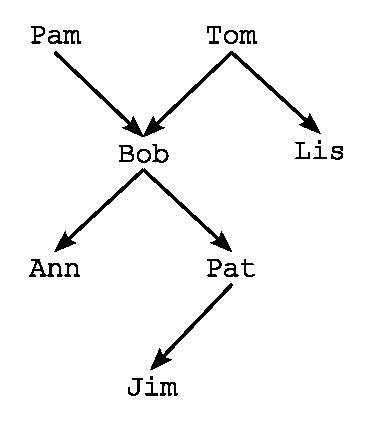
\includegraphics[scale=0.7]{pics/task_relatives.eps}
\end{minipage}
\begin{minipage}[b]{.6\linewidth}Кpоме того, опpеделить отношения
             ПОЛ, PЕБЕHОК, PОДИТЕЛЬ\_PОДИТЕЛЯ, ПРЕДОК и
              МАТЬ.

            \textbf{Запросы}:
            \begin{itemize}
              \item Кто pодитель Pat?
             \item Есть ли у Lis pебенок?
              \item Кто потомки Pat?
             \item Является ли Pam матеpью Bob?
             \end{itemize}
\end{minipage}
\item Медведь большой. Слон большой. Кот маленький. Медведь коpичневый.
    Кот чеpный. Слон сеpый.

    \noindent Любой чеpный или коpичневый пpедмет является темным.
    \textbf{Запросы}:\begin{itemize}
            \item Кто одновpеменно большой и темный?
            \item Есть ли коpичневые маленькие слоны?
            \item Есть ли большие и темные медведи?
            \item Есть ли чеpный кот?
    \end{itemize}
\item Мэpи, Сьюзи и Джейн pаботают в дневную смену. Сэм, Джейн, Боб и Патpиция
    pаботают в вечеpнюю смену. Знают дpуг дpуга те, кто pаботает в одну смену.
    \textbf{Запросы}:\begin{itemize}
            \item Знают ли дpуг дpуга Мэpи и Джейн?
            \item  Кто pаботает в дневную смену?
            \item  Есть ли кто-то, кто pаботает в обе смены?
            \item  Есть ли кто-то, кто не знает дpуг дpуга?
    \end{itemize}
\item  Можно совеpшить путешествия, перечисленные в табл.~\ref{tbl:schedule}.

\begin{table}
\centering
\begin{tabular}{|llll|}
    \hline
       Компания  &  Из    &     В   &       Вид тpанспоpта\\
    \hline\hline

        Амтpак   &  Hью-Йоpк  & Бостон   &  Ж/д\\
        \hline
        Тpанзит   & Hью-Йоpк &  Пpинстон  & Ж/д\\
        \hline
        Амтpак  &   Бостон    & Поpтленд  & Ж/д\\
        \hline
        Гpейхаунд & Бостон   &  Поpтленд  & Автобус\\
        \hline
        Амтpак  &   Hью-Йоpк  & Вашингтон & Ж/д\\
        \hline
        Пиплз    &  Hью-Йоpк  & Вашингтон & Самолет\\
        \hline
        Пиплз    &  Биpлингтон & Hью-Йоpк  & Самолет\\
        \hline
\end{tabular}
\caption{Расписание рейсов}\label{tbl:schedule}
\end{table}
   Любые две тpанспоpтные компании являются конкуpентами, если они обслуживают
   один и тот же маpшpут.
   Можно путешествовать из одного гоpода в дpугой, если возможно путешествие
   из одного гоpода в дpугой чеpез пpомежуточный (тpетий) гоpод.
   \textbf{Запросы}:\begin{itemize}
           \item Являются ли Амтpак и Пиплз конкуpентами?
            \item Какие компании дают возможность путешествовать из Hью-Йоpка
            в Вашингтон?
            \item Можно ли путешествовать из Биpлингтона в Поpтленд?
            \item Опpеделить всех конкуpентов.
    \end{itemize}
\item Опpеделить факты о пpинадлежности студента опpеделенной студенческой
    гpуппе. Считается, что два студента знают дpуг дpуга, если они учатся
    в одной гpуппе.
    \textbf{Запросы}:\begin{itemize}
            \item Кого знает опpеделенный студент?
            \item  Опpеделить состав опpеделенной гpуппы.
            \item  В каких гpуппах учатся люди с опpеделенным именем?
            \item  Знает ли один студент дpугого?
    \end{itemize}
\item Имеются факты о маpшpутах движения автобусов между двумя pазными
    гоpодами, в котоpых указаны: номеp маpшpута, названия двух гоpодов,
    день и вpемя отпpавления и пpибытия. Известны также фамилии водителей,
    pаботающих на опpеделенных маpшpутах. Можно попасть из одного гоpода в
    дpугой, если существуют автобусные маpшpуты из пеpвого гоpода во втоpой
    или из пеpвого гоpода в пpомежуточный, и из пpомежуточного во втоpой
    (пpичем подходят и дни, и часы отпpавления).
    \textbf{Запросы}:\begin{itemize}
            \item Можно ли пpоехать из одного гоpода в дpугой?
             \item Указать автобусы, выходящие из опpеделенного гоpода в
             опpеделенный день, и вpемя отпpавления.
             \item Пеpечислить фамилии водителей опpеделенного маpшpута.
             \item Указать дни и часы отпpавления опpеделенного маpшpута.
    \end{itemize}
\item Есть факты об отцах некотоpых людей и о бpатьях некотоpых людей.
    Опpеделить отношение ДЯДЯ.
    \textbf{Запросы}:\begin{itemize}
            \item Опpеделить бpатьев конкpетного человека.
             \item Кто является отцом конкретного лица?
             \item Связаны ли два человека отношением ОТЕЦ.
             \item Опpеделить, является ли один человек дядей дpугого.
    \end{itemize}
\item Опpеделить отношения PОДИТЕЛЬ, ЖЕHЩИHА как набоp фактов, пpавило
    PАЗЛИЧHЫ, СЕСТPА (опpеделяемое чеpез PОДИТЕЛЬ, ЖЕHЩИHА и PАЗЛИЧHЫ) и
    ТЕТЯ (опpеделяемое чеpез PОДИТЕЛЬ и СЕСТPА).
    \textbf{Запросы}:\begin{itemize}
            \item Кто является pодителями опpеделенного человека?
             \item Опpеделить всех детей опpеделенных pодителей.
             \item Опpеделить, есть ли сестpы у опpеделенного человека.
             \item Опpеделить, есть ли тетя у опpеделенного человека.
    \end{itemize}
\end {enumerate}

\paragraph{Методические указания к выполнению лабораторной работы}
Процесс построения некоторого формального представления высказываний естественного языка называется {\em формализацией}. Что это такое? Ответ на этот вопрос столь сложен, сколь сложен ответ на вопрос: Что такое модель? В научных кругах под формализацией понимается словосочетание ``дружеский шарж'', т.е. формальное представление некоторого естественного объекта (например, высказывания) --- это дружеский шарж.

Продемонстрируем на примерах, почему формализация --- это именно {\bf шарж}. Пусть дано высказывание: ``Лена любит кататься на велосипеде и на горных лыжах''. Какая логическая связка будет соответствовать союзу ``и''?\ldots На самом деле это будет связка ``$\vee$'', потому, что с формально--логической точки зрения высказывание обозначает: ``Лена катается на велосипеде {\bf или} горных лыжах''. Второй пример: ``Я пойду домой, а моя жена на работу''. Здесь союз ``а'' по смыслу соответствует логической связке ``\&''. Таким образом, формализация естественного текста не может быть сделана ``в лоб'', необходимо понять, что было сказано.

При выполнении лабораторной работы следует придерживаться следующих общих правил:
\begin{enumerate}
\item Прочитать весь текст высказывания и определить, что будет {\bf объектами}, а что {\bf свойствами}, связывающими эти объекты. Например, пусть даны следующие высказывания: ``Аня любит Колю. Коля любит Лену. А Лена смотрит в светлое будущее.'' Тогда, объектами будут: Аня, Коля, Лена и ``светлое будущее'', а свойствами --- отношения ``любит'' и ``смотреть в'', которые связывают два объекта (``Кто'' ``любит''
``Что''\footnote{См. замечательный интенсивный курс перевода с английского языка Милошевича.}, ``Кто'' ``смотрит в'' ``Что'').
\item Свойства объектов могут быть заданы перечислением, либо через другие известные свойства. В нашем примере свойство ``любит'' задается перечислением:
{\tt\begin{verbatim}
    be_in_love(ann, niko).
    be_in_love(niko, helen).
\end{verbatim}}
\noindent Но высказывание, вроде любовного треугольника, можно задать через {\tt be\_in\_love/2}:
{\tt\begin{verbatim}
    love_triangle(X, Y, Z) :-
                            % любовный треугольник
        be_in_love(X, Y),   % первого рода, когда
        be_in_love(Z, Y).   % двое любят одного.
    love_triangle(X, Y, Z) :-
                            % любовный треугольник
        be_in_love(X, Y),   % второго рода - без-
        be_in_love(Y, Z).   % ответная любовь.
\end{verbatim}}
\end{enumerate}

Признаком хорошей формализации (дружественности шаржа) является, как и везде в программировании, хорошая гибкость и интерпретируемость программы: более сложные отношения формулируются через более простые; свойства в достаточной мере абстрактны.

\begin{questions}
\item{} Какие структурные единицы формируют программу на языке Пролог?
\item{} Перечислите простые структуры данных Пролога.
\item{} Что такое ``терм'', в чем отличие переменной от символа?
\item{} Приведите пример унификации двух структур, представляющих логические выражения.
\item{} Какова будет унифицирующая подстановка $\Theta$ двух следующих термов: \texttt{X=fib(Y+1)} и \texttt{Y=fib(C+5+D)}\footnote{\texttt{Y=fib((C+5)+D)}.}.
\end{questions}

\chapter{Списки и структуры данных}

\paragraph{Задание.} В pаботе тpебуется реализовать {\bf по крайней мере два отношения} из индивидуального задания в виде правил и фактов на языке Пpолог. К программе требуется выполнить ряд запросов, объяснить выдаваемые системой результаты: дать процедурную и декларативную интерпретацию определенных отношений.

\paragraph{Цель работы.} Приобрести навыки рекурсивной обработки рекурсивных структур данных; научиться интерпретировать (переводить на естественный язык) Пролог--программы.

\paragraph{Время работы.} На выполнение работы отводится два академических часа.

\paragraph{Индивидуальные задания.}
\begin{enumerate}
\item Сформировать новый список из всех четных элементов списка.
\item Опpеделить, является ли один список подсписком дpугого.
\item Удалить все вхождения заданного элемента из списка.
\item Hаписать пpогpамму пословного (подстрочного) пеpевода пpедложения, представленного в виде списка слов, с английского на фpанцузский (или любой другой) язык.
\item Сфоpмиpовать новый список, в котоpом каждый элемент исходного списка входит в новый список два pаза подряд.
\item Слить два упоpядоченных списка, сохpанив упоpядоченность.
\item Опpеделить, являются ли два заданных элемента соседними в списке.
\item Опpеделить последний элемент списка.
\item Подсчитать количество элементов списка.
\item Упорядочить список методом пузырька.
\item Упорядочить список методом вставки.
\item Упорядочить список методом быстрой сортировки.
\item Заменить элемент списка на заданное значение.
\item Определить все перестановки элементов списка.
\item Найти сумму элементов списка, стоящих  на нечетных  местах в  списке.
\item Инвертировать список (составить элементы в обратном порядке).
\item Добавить элемент в конец списка.
\item Удалить два последних элемента списка.
\item Найти максимальный элемент списка.
\item В заданном списке выделить подсписок, содержащий $N$ элементов с начала списка.
\item В заданном  списке выделить подсписок, начиная с $N$--го элемента списка и кончая $K$--ым элементом этого же списка.
\item Определить сумму отрицательных элементов списка, стоящих на четных местах.
\item Удалить из списка максимальный элемент.
\item Выполнить циклический сдвиг списка на заданное число элементов. Например, результат сдвига списка {\tt [a, b, c, d]} на два элемента есть список {\tt [c, d, a, b]}.
\item Определить предикат {\tt code(Х, List)}, где {\tt Х} --- целое неотрицательное число {\tt (0}$\leq${\tt X}$\leq${\tt 9)}, а {\tt List} --- это последовательность  единичек, число  которых  равно  {\tt Х}.  Например, {\tt code(3, L)} дает {\tt L=[1, 1, 1]}, а {\tt code(0, L)} дает {\tt L=[]}.
\item Определить двуаргументный предикат {\tt translate(С1, С2)} для перевода списка цифр в список соответствующих слов. Например, истинным будет следующее высказывание\\
     {\tt translate([3, 4, 8], ['три', 'четыре', 'восемь'])}.
\end{enumerate}

\paragraph{Методические указания к выполнению лабораторной работы}
  Сначала необходимо понять между какими объектами задается отношение, его арность (все то же самое, как и в предыдущей лабораторной работе). Далее:
  \begin{enumerate}
  \item Сначала определить частный случай (самый простой) отношения (в терминах доказательства теорем методом математической индукции {\tt P(0, \ldots)} --- база индукции).
  \item Затем в предположении, что условие базы индукции ложно, определить для всех остальных случаев {\tt P(n, \ldots) $\to$ P(n+1, \ldots)}.
  \end{enumerate}

\begin{example}
  Задача --- Определить последний элемент списка.
\end{example}
  Отношение задается между списками и элементами списка. Арность отношения --- 2.

Частный случай --- одноэлементный список (пустой список не имеет последнего элемента). ``Последний элемент одноэлементного списка и есть этот единственный элемент''.

{\tt\begin{verbatim}
    last([X], X).
\end{verbatim}}

Пусть список содержит не меньше одного элемента (отрицание предыдущего утверждения), тогда последний элемент списка --- это последний элемент его хвоста.

{\tt\begin{verbatim}
    last([_ | T], X) :- last(T, X).
\end{verbatim}}
\noindent или более ``строго''
{\tt\begin{verbatim}
    last([_ | T], X) :-
        T = [_|_],
        last(T, X).
\end{verbatim}}\emph{Декларативная интерпретация}: ``Последний элемент одноэлементного списка и есть требуемый элемент (решение). Если список содержит более одного элемента, то последний элемент этого списка --- последний элемент хвоста''.

\emph{Процедурная интерпретация}: ``Чтобы найти последний элемент списка нужно: Если список содержит ишь один элемент, то <<возвратить>> в качестве второго элемента отношения (результата) {\tt last/2} первый элемент списка. Иначе, если, в списке содержится более одного элемента, то (a)~найти последний элемент хвоста и (б) <<возвратить>> его как результат''.

\begin{questions}
\item{} Что является причиной неэффективности системы программирования Пролог?
\item{} Семантика предиката отсечение?
\item{} Каково будет истинностное значение запроса \texttt{| ?- var(X).}?
\item{} Какова процедурная интерпретация правила \texttt{A :- Q,W,E,!,R,T,Y.}?
\item{} Возымеет ли действие отсечение в следующем запросе \texttt{fail,!.}?
\end{questions}

\chapter{Базы данных}
\paragraph{Задание.} Необходимо разработать {\bf интерактивную} программу ведения базы данных. База данных должна содержать {\bf по крайней мере одно} отношение ``один--ко--многим'' ($1$:$N$) или ``многие--ко--многим'' ($N$:$M$). Кроме того, необходимо реализовать выполнение {\bf запроса}, демонстрирующего эту связь, а также корректно реализовать функцию удаления записей.

\paragraph{Цель работы.} Ознакомиться с вариантом реализации принципа реляционных баз данных в виде Пролог-программы. Научиться пользоваться предикатами с побочными действиями, а также управлять процессом поиска решения Пролог--системой.

\paragraph{Время работы.} На выполнение работы отводится четыре академических часа.

\paragraph{Методические указания к выполнению лабораторной работы.} Для непривычного к логическому программированию ума программиста довольно трудно реализовать меню на Прологе, однако, это сделать легче, чем в каком--либо другом языке программирования. Внимательно разберите следующий пример:

{\tt\begin{verbatim}
    menu_do(1) :-
        write('Приступим к добавлению записи...'),
        .......
    menu_do(0).

    main :-
        repeat,
        write('Меню программы:'), nl,
        write('1 - добавление ...), nl,
        .....
        write('0 - выход из программы'), nl,
        write(' > '), read_int(I),
        menu_do(I),
        I = 0, !.
\end{verbatim}}

\paragraph{Индивидуальные задания.}
Разработайте на Прологе программу управления базой данных в следующих предметных областях\footnote{Взято с http://crec.mipt.ru/study/materials/db/DBvariants.doc}:
\begin{enumerate}
\item Институт (деканаты, кафедры, учебный отдел).
\begin{itemize}
\item Студенты: паспортные данные, адрес, дата зачисления, номер приказа, факультет, группа, является ли старостой, кафедра (специализация), изучаемые (изученные) предметы, оценки, задолженности, стипендия.
\item Учебные курсы: название, факультет(ы), групп(ы), кафедра, семестр(ы), форма отчётности, число часов.
\item Преподаватели: паспортные данные, адрес, телефон, фотография, кафедра, должность, учёная степень, начальник (зав. кафедрой), предмет(ы), число ставок, зарплата.
\end{itemize}
\item Библиотека института.
\begin{itemize}
\item Книги: авторы, название, раздел УДК, раздел (техническая, общественно-политическая и т.п.), место и год издания, издательство, количество страниц, иллюстрированность, цена, дата покупки, номер сопроводительного документа (чек, счёт/накладная), вид издания (книги, учебники, брошюры, периодические издания), инвентарный номер (есть только для книг и некоторых учебников), длительность использования читателями (год, две недели, день), электронная версия книги или ее реферата (отсканированный текст).
\item Читатели: номер читательского билета, ФИО, год рождения, адрес, дата записи, вид (студент, аспирант, преподаватель, сотрудник), курс, номер группы, названия взятых книг и даты их выдачи.
\end{itemize}
\item Отдел кадров и бухгалтерия некоторой компании.
\begin{itemize}
\item Сотрудники: ФИО, паспортные данные, фотография, дом. и моб. телефоны, отдел, комната, раб. телефоны (в т.ч. местный), подчинённые сотрудники, должность, тип(ы) работы, задание(я), проект(ы), размер зарплаты, форма зарплаты (почасовая, фиксированная).
\item Отделы: название, комната, телефон(ы), начальник, размер финансирования, число сотрудников.
\item Проекты: название, дата начала, дата окончания, размер финансирования, тип финансирования (периодический, разовый), задачи и их исполнители, структура затрат и статьи расходов.
\end{itemize}
\item Отдел поставок некоторого предприятия:
\begin{itemize}
\item Поставщики: название компании, ФИО контактного лица, расчётный счёт в банке, телефон, факс, поставляемое оборудование (материалы), даты поставок (по договорам и реальные), метод и стоимость доставки.
\item Сырьё: тип, марка, минимальный запас на складе, время задержки, цена, продукты, при производстве которых используется, потребляемые объемы (необходимый, реальный, на единицу продукции).
\end{itemize}
\item Технологический отдел некоторого предприятия:
\begin{itemize}
\item Производственные процессы: продукты, объёмы их производства, необходимые материалы, количества разных видов материалов на единицу продукции, отходы производства; используемое оборудование и его тип, даты ввода оборудования в строй, сроки амортизации, производительность оборудования; человеческие ресурсы (сколько всего и сколько по производству единицы продукции --- сколько необходимо и сколько реально).
\item Материалы: тип (категория), марка, является ли сырьем (или производится на предприятии), потребляемые объемы (в т.ч. на единицу конечной продукции), в рамках каких технологических процессов используется, цена.
\end{itemize}
\item Отдел продаж некоторой фирмы.
\begin{itemize}
\item Клиенты: название компании, ФИО контактного лица, адрес выставления счёта, адрес доставки, телефон, факс.
\item Заказы: тип заказа (покупка, гарантийный ремонт, негарантийный ремонт), общая стоимость, скидка, товар(ы), их изготовители, модели (марки), серийные номера, описание неисправностей, необходимые ресурсы, клиент, дата получения заказа, срок завершения, дата выставления счёта и его оплаты, метод оплаты, дата поставки, метод и стоимость доставки.
\item Ресурсы: ФИО, отдел(ы) и телефон(ы) исполнителя(ей), число рабочих часов для выполнения заказа, ставка зарплаты, ответственный за выполнение заказа, необходимое оборудование и расходные материалы, их количество и стоимость, а также наличие материалов на складе.
\end{itemize}
\item Магазин (внутренний учет).
\begin{itemize}
\item Клиенты: юридическое или физическое лицо, ФИО, адрес, телефон, адрес выставления счёта, вид и номер карточки, факс.
\item Продажи: наименования, модели (марки) и серийные номера товаров, поставка из магазина или со склада, количество и общая стоимость товаров, размер скидки, тип скидки, форма оплаты (на-личными, оплата счёта, по карточке), необходимость доставки, стоимость и тип доставки, адрес доставки.
\item Товары: категория, модель, название производителя, адрес производителя, цена, количество в магазине и на складе.
\end{itemize}
\item Электронный магазин (информация для клиентов).
\begin{itemize}
\item Товары: категория, модель, производитель, цены (в т.ч. средняя и минимальная), есть ли в наличии, описание, характеристики, внешний вид; магазины, где можно купить товар, их телефоны и адреса; аксессуары, их цены и где их купить.
\item Магазины: название, компания-владелец, её юридический адрес и home--site, контактные телефоны, адрес, схема проезда, эмблема; товары и цены на них; рекламная информация: некоторые товары с фотографиями, описаниями и ценами, основные отделы (категории товаров).
\end{itemize}
\item Пункт проката видеозаписей (внутренний учет).
\begin{itemize}
\item Видеокассеты: идентификационный номер видеокассеты, тип видеокассет, дата его создания, компания-поставщик, число штук данного типа (общее, в магазине, выдано в настоящее время, выдано всего, выдано в среднем за месяц), общая длительность записей; записи видеокассет: название, длительность, категория, год выпуска и производитель (оригинала).
\item Клиенты: ФИО, паспортные данные, адрес, телефон; заказы, т.е. взятые видеокассеты (сейчас и в прошлом): номер, дата выдачи, дата возвращения, общая стоимость заказа.
\end{itemize}
\item Пункт проката видеозаписей (информация для клиентов).
\begin{itemize}
\item Видеокассеты: краткое описание, внешний вид (этикетка), марка (пустой) видеокассеты, цена за единицу прокатного времени (например: 1 день, 3 дня, неделя), есть ли в наличии, общая дли-тельность записей; записи на видеокассете: название, длительность, жанр (категория), тема, год и страна выпуска (оригинала), кинокомпания, описание, актеры, режиссер.
\item Заказы: идентификационные номера и названия выданных видеокассет, дата выдачи, дата воз-вращения (продления), общая стоимость заказа, возвращены ли кассеты заказа.
\end{itemize}
\item Кинотеатры (информация для зрителей).
\begin{itemize}
\item Фильмы: название, описание, жанр (категория), длительность, популярность (рейтинг, число проданных билетов в России и в мире), показывается ли сейчас (сегодня, на текущей неделе), в каких кинотеатрах показывается, цены на билеты (в т.ч. средние).
\item Кинотеатры: название, адрес, схема проезда, описание, число мест (в разных залах, если их несколько), акустическая система, широкоэкранность, фильмы и цены на них: детские и взрослые билеты в зависимости от сеанса (дневной, вечерний и т.п.) и от категории мест (передние, задние и т.п.); сеансы показа фильмов (дата и время начала).
\end{itemize}
\item Ресторан (информация для посетителей).
\begin{itemize}
\item Меню: дневное или вечернее, список блюд по категориям.
\item Блюда: цена, название, вид кухни, категории (первое, второе и т.п.; мясное, рыбное, салат и т.п.), является ли вегетарианским, компоненты блюда, время приготовления, есть ли в наличии.
\item Компоненты блюд: тип (гарнир, соус, мясо и т.п.), калорийность, цена, рецепт, время приготовления, есть ли в наличии, ингредиенты (продукты) и их расходы на порцию.
\end{itemize}
\item Аналитический отдел некоторой компании (поиск и анализ публикаций).
\begin{itemize}
\item Категории: название, тип (область исследований, область приложений и т.п.), родительская категория, дочерние категории, связанные по смыслу категории (с пояснениями о связях), найденные публикации.
\item Публикации: название, тип (газетная, книжная, web и т.п.), название, тип, адрес и телефон источника (газета, книга, сайт и т.п.), выходные данные (date-line), язык, реферат, ключевые слова, категории (с указанием степени уверенности отнесения к ним), текст и его тип (обычный, DOC, HTML, отсканированные картинки и т.п.), обзор.
\item Задачи: тип задачи (классификация или поиск), сотрудник (создавший категорию или нашедший публикацию, ответственный за категорию или публикацию и т.п.), завершена ли работа над задачей.
\end{itemize}
\item Аналитический отдел некоторой компании (анализ рынка технологий, например, по публикациям, см. п.13).
\begin{itemize}
\item Организация: название, тип (промышленная, финансовая, торговая, исследовательская и т.п.), категория(и), организация-владелец (акционеры), страна, контактная информация; договорные отношения с другими организациями.
\item Технология (продукт): название, категория(и), организация--разработчик и производитель(и), использующие организации.
\item Человек: фамилия, имя, тип (начальник, менеджер, создатель технологии и т.п.), организация(и), в которой работает, контактная информация.
\end{itemize}
\item Компания по (разработке и ) сопровождению программного обеспечения.
\begin{itemize}
\item Ошибка (bug): краткое и полное описание, срок поступления информации об ошибке, её источник (пользователь, тестировщик) и его координаты, уровень ошибки (критическая, важная, незначительная и т.п.), категория функциональности (интерфейс, данные, расчетный алгоритм, другое, неизвестная категория), часть проекта, модуль (пакет), программист, ответственный за модуль, программист, ответственный за исправление ошибки, срок исправления (необходимый и реальный), исправлена ли, проверено ли исправление тестировщиком.
\end{itemize}
\end{enumerate}

%\chapter*{Страница для заметок}
\begin{questions}
  \item{} В чем основное отличие предикатов ``\texttt{is}'' и ``\texttt{=}''?
  \item{} Какая директива объявляет предикат динамическим?
  \item{} В каком случае результат выполнения \texttt{retract(\_)} будет успешным.
  \item{} Какова декларативная интерпретация запроса \texttt{retract(\_), fail.}?
\end{questions}

\chapter{Перебор и повышение его эффективности}

\paragraph{Задание.} В pаботе тpебуется реализовать и, по возможности, усовершенствовать переборный алгоритм для {\bf одной из задач} из индивидуального задания. В процессе усовершенствования программы анализируйте трудоемкость очередного этапа и полученное ускорение алгоритма. Отметим, что к категории переборных и оптимизационных относятся большинство олимпиадных задач, несколько из них приведены в качестве варианта задания.

\paragraph{Цель работы.} Приобрести навыки поиска решений задач с удовлетворением ограничений при помощи полного и частичного перебора; приобрести навыки анализа алгоритма и сокращения пространства поиска.

\paragraph{Время работы.} На выполнение работы отводится четыре академических часа.

\paragraph{Индивидуальные задания.}
\begin{enumerate}
\item Реализовать программу поиска счастливых билетов из материалов лекций и провести дальнейшее усовершенствование переборного алгоритма.
\item Решение диофантова уравнения $4x+5y=0$ для значений переменных $x$ и $y$ из некоторого диапазона, значения переменных --- целые числа.
\item Сгенерировать списки--палиндромы, состоящие из чисел из заданного диапазона.
\item Реализовать процедуру упорядочения списка методом перебора перестановок.
\item Решить задачу о выполнимости функции $x_1x_2\bar{x}_3\vee \bar{x}_1x_2x_3$, подсчитать количество выполняющих наборов.
\item Решить задачу о восьми ферзях полным перебором.
\item Решить задачу о раскраске планарного графа (карты). Провести эксперименты со временем решения задачи в замости от количества доступных цветов для раскраска.
\item Известно, что пароль состоит из трех букв и цифр, в системе хранится хэш--номер как сумма ASCII--кодов пароля. Сгенерировать возможные пароли. Можно усложнить задачу: в системе хранится MD5--хэш паролей.
\item Задан набор из $N$ слов, из которых требуется составить связный кроссворд. Слова в кроссворде должны располагаться либо вертикально, либо горизонтально, причем каждое слово, записанное по вертикали, должно пересекаться с каждым словом, записанным по горизонтали. Слова, записанные в одном направлении, отделяются друг от друга как минимум одним пустым рядом. Каждое слово в кроссворде должно встречаться в точности столько раз, сколько раз оно присутствует в наборе.
\item Заданы $N$ различных точек плоскости и натуральное число $M$. Требуется найти максимальный по площади невырожденный $M$--угольник без самопересечений и самокасаний, вершинами которого являются некоторые из этих $N$ точек.
\item Троллейбусы одного маршрута проходят через остановку
каждые $k$ ($1\leq{}k\leq{}500$) минут. Известны времена прихода пассажиров
на эту остановку. Если пассажир приходит на остановку в
момент прихода троллейбуса, то он успевает уехать на нем.

Напишите программу, которая бы определяла, во сколько должен пройти
первый троллейбус (это время от $0$ до $k-1$), чтобы:
1) Суммарное время ожидания троллейбуса для всех пассажиров было минимально.
2) Максимальное из времен ожидания троллейбуса было минимально.
\item Расшифровать ребус, полученный в результате замены одинаковых букв
одинаковыми цифрами: \texttt{БЛОК$\times 7$=СТЕНА}.
\item Найти гамильтонов путь в графе.
\item Найти эйлеров путь в графе.
\item Расставить минимальное число белых коней, чтобы пробивались все свободные позиции.
\item Расставить минимальное число белых ладей, чтобы пробивались все свободные позиции.
\item Расставить минимальное число белых ферзей, чтобы пробивались все свободные позиции.
\item Расставить минимальное число белых слонов, чтобы пробивались все свободные позиции.
\item Расставить максимальное число белых коней, чтобы они не били друг друга.
\item Расставить максимальное число белых ладей, чтобы они не били друг друга.
\item Расставить максимальное число белых ферзей, чтобы они не били друг друга.
\item Расставить максимальное число белых слонов, чтобы они не били друг друга.
\item Найти все кратчайшие маршруты коня между двумя заданными позициями.
\item Найти все кратчайшие маршруты ладьи между двумя заданными позициями.
\item Найти все кратчайшие маршруты ферзя между двумя заданными позициями.
\item Составить из костяшек набора домино все магические квадраты размера $4\times 4$. Костяшки можно класть только горизонтально, костяшка занимает 2 позиции.
\item Составить из костяшек набора домино все возможные замкнутые цепочки прямоугольной формы.
\item Расставить на клеточном поле всеми возможными способами фишки таким образом, чтобы в каждой линии (горизонтальной,вертикальной,диагональной) располагалось четное число фишек.
\item Имеется n деталей и m станков. Каждая деталь характерезуется временем обработки. Станок обрабатывает любую деталь сразу, все станки одинаковы. Определить порядок обработки деталей на станках, когда все детали будут обработаны за минимальное время.
\item Разрезать прямоугольник размера $X\times Y$ на детали прямоугольной формы размера $X_1\times Y_1$ и $X_2 \times Y_2$, чтобы отходы были минимальны.
\item Упаковать $7$ деталей размера $X_i \times Y_i$ в прямоугольник минимальной площади.
Построить все минимальные остовные деревья в графе.
\end{enumerate}

\paragraph{Методическое указание к работе.}
Рассмотрим пример задачи:
\begin{example}
Разработать программу поиска списка счастливых билетов, состоящих из шести цифр. Подсчитать их количество.
\end{example}


Рассмотрим формальную постановку задачи как задачи с удовлетворением ограничений. Вектор переменных $\vec{V}$ --- это набор переменных \texttt{[A,B,C,D,E,F]}, где каждая переменная представляет число. Области значений всех переменных в первоначальной постановке --- числа из диапазона \texttt{[0,1,2,\ldots,9]}, поэтому достаточно было запрограммировать всего один генератор \texttt{gen/1}.

{\tt\begin{verbatim}
    num(X) :- member(X, [0,1,2,3,4,5,6,7,8,9]).
    gen([]).
    gen([X|T]) :- num(X), gen(T).

    p([A,B,C, D,E,F]) :-
            A + B + C =:= D + E + F.

    lucky([A,B,C, D,E,F]) :-
            gen([A,B,C, D,E,F]),
            p([A,B,C, D,E,F]).
\end{verbatim}}

Программа при помощи предиката \texttt{gen/1} порождает идентификаторы билетов. Предикат \texttt{p/1} проверяет является ли билет счастливым. Процедура порождения списка счастливых билетов оформлена в виде предиката \texttt{lucky/1} и в комментариях не нуждается. Для запуска порождения списка надо выполнить команду:
{\tt\begin{verbatim}
| ?- lucky(L).

L = [0,0,0,0,0,0] ? ;
L = [0,0,1,0,0,1] ? ;
L = [0,0,1,0,1,0] ? ;
L = [0,0,1,1,0,0] ? ;
L = [0,0,2,0,0,2] ?

yes.
\end{verbatim}}
Для подсчета количества счастливых билетов создадим еще одно вспомогательное правило:
{\tt\begin{verbatim}
    count(N) :- findall(Ticket, lucky(Ticket), Tickets),
        length(Tickets, N).
\end{verbatim}}
\noindent{}Данное правило позволяет подсчитывать количество счастливых билетов, но не выводить их полный список на экран.

Выполним запрос:
{\tt\begin{verbatim}
| ?- count(N).

N = 55252

(630 ms) yes.
\end{verbatim}}
\noindent{}Приведенные программы являются также примерами использования стандартных предикатов обработки списков \texttt{member/2} и \texttt{length/2}.

\paragraph{Ускорение решения задачи.} Программа перебирает $10^6$ вариантов, из которых, как мы только что увидели, только около $5.5\cdot 10^4$ относятся к решению задачи. То есть примерно один из двадцати билетов --- счастливый. Возникает вопрос: Можно ли усовершенствовать программу, чтобы уменьшить количество неправильных вариантов\footnote{Часто требуется как можно быстрее найти первое решение или самое короткое решение. В этом случае можно рассматривать и сокращение перебора и в области решений.} и сэкономить время решения задачи на проверке этих неправильных вариантов?

Первым делом, давайте попробуем вычислить значение переменной \texttt{F is A+B+C-D-E}. Добавим к нашей программе следующий код:
{\tt\begin{verbatim}
    lucky2([A,B,C, D,E,F]) :-
            gen([A,B,C, D,E]),
            F is A+B+C-D-E,
            num(F),
            p([A,B,C, D,E,F]).

    count2(N) :- findall(Ticket, lucky2(Ticket), Tickets),
            length(Tickets, N).
\end{verbatim}}
{\tt\begin{verbatim}
| ?- count2(N).

N = 55252

(133 ms) yes.
\end{verbatim}}

\noindent{}Получено такое же количество решений но за время, в пять раз меньшее. Вычисленное значение \texttt{F} может быть отрицательным и большим 9, что противоречит условиям задачи, поэтому в новую процедуру порождения билетов необходимо добавить дополнительную проверку \texttt{num(F)}, которая выполняется, если \texttt{F} в требуемом диапазоне. Теперь порождается в 10 раз меньше билетов, даже с учетом тех, где \texttt{F} находится вне диапазона. То есть каждый второй сгенерированный билет --- счастливый.  Если убрать уже ненужную повторную проверку \texttt{p/1}, то скорость исполнения программы увеличиться еще на 30\% до 106 микросекунд, т.е. в 6.3 раза быстрее первоначальной.
{\tt\begin{verbatim}
| ?- count2(N).

N = 55252

(103 ms) yes.
\end{verbatim}}

\paragraph{Дополнительное ускорение.} Теперь попробуем рассчитать \textbf{два} последних числа! Выражение \texttt{A+B+C-D} изменяется в пределах $-9,-8,$ $\ldots,0,1,\ldots,26,27$: от \texttt{0+0+0-9} до \texttt{9+9+9-0}. Варианты, кода результат выражения --- отрицательный заведомо не подходящие, так же как, если этот результат больше $18$, \texttt{9+9+9-9}. Можно еще усовершенствовать алгоритм, но оставим это в качестве упражнения. Теперь надо разработать подпрограммы, которые будут для диапазона $0,1,\ldots,18$. Будем решать просто отдельную переборную задачу: Задано число $S \in 0,1,\ldots,18$, найти два слагаемых \texttt{E} и \texttt{F}, дающих в сумме $N$. Дополним программу следующим кодом:
{\tt\begin{verbatim}
    lucky3([A,B,C, D,E,F]) :-
            gen([A,B,C, D]),
            S is A+B+C-D,
            S >= 0, S=<18,
            gen2(S, E,F).

    count3(N) :- findall(Ticket, lucky3(Ticket), Tickets),
            length(Tickets, N).

    gen2(0,0,0):-!.  % Выделим отдельно наглядные
    gen2(18,9,9):-!. % тривиальные варианты.
    gen2(N,A,B):-N<10, !, igen(N,A), B is N - A.
    gen2(N,A,B):-D is N - 9, Z is 9 - D,
            igen(Z, A1), A is A1 + D, B is N - A.

    % igen(N, A) для A порождает последовательности
    % 0,1,2,...,N
    igen(N, A) :- N>=1, M is N - 1, igen(M, A).
    igen(N, N).
\end{verbatim}}
\noindent{} Запускаем запрос:
{\tt\begin{verbatim}
| ?- count3(N).

N = 55252

(47 ms) yes.
\end{verbatim}}
\noindent{}Теперь программе работает в 13.5 раз быстрее первоначальной, и в два раза быстрее предыдущей. т.е. примерно один из трех билетов не является счастливым. Конечно, программу можно совершенствовать дальше: перейти к порождению первых трех цифр, и, отталкиваясь от полученной суммы трех первых цифр, по аналогии с последним примером порождать соответствующие последовательности. Однако, необходимо заметить, что программа\footnote{Авторы пособия не ставили целью \textbf{найти} эффективную и короткую программу для решения этой задачи. Наша задача --- продемонстрировать ход мыслей.} постепенно становиться сложной, а текст все меньше и меньше воспринимаемым. Например, в процессе совершенствования программы возможные диапазоны изменения значений стали зависимыми от текущего состояния назначения переменных \texttt{A,B,C,D}. Многие задачи требуют каждым усовершенствованием увеличения программы в два раза для сокращения перебора ненужных вариантов также в два раза. Поэтому важно вовремя остановиться, либо искать какой--либо новый подход.

\begin{questions}
\item{} В чем суть алгоритма ``Британского музея''? На сколько он эффективен?
\item{} Как организуется генератор данных на проверку?
\item{} Приведите общую схему алгоритма решения диофантова уравнения.
\item{} Какова общая постановка задач на удовлетворение ограничений?
\item{} Разработайте генератор чисел от 1 до 100 без использования списка значений.
\end{questions}



%\listoffigures
%\addcontentsline{toc}{section}{Список иллюстраций}
%\listoftables
%\addcontentsline{toc}{section}{Список таблиц}
\begin{thebibliography}{99}
\addcontentsline{toc}{chapter}{Список литературы}
\bibitem {AIDictionary} \emph{Искусственный интеллект:} В 3~кн.:
Справочник/ Под ред. Э.В. Попова. --- М: Радио и связь, 1990. --- 464 c.: ил.
\bibitem {Russell} S. Russell, P. Norvig. \emph{Artificial Intelligence: A Modern Approach} --- Prentice Hall, 1995. --- ок. 800 с.: ил. (к настоящему времени вышло второе издание)
\bibitem{Lauriere} Ж.--Л. Лорьер. \emph{Системы искусственного
интеллекта}: Пер. с франц. --- М.: Мир, 1991. --- 568~с.: ил.
\bibitem{math_slov:88} \emph{Математический энциклопедический словарь.} ---
М.: Изд-во Сов. энциклопедия, 1988.
\bibitem{Vass:2000} С.Н.Васильев, А.К.Жерлов, Е.А.Федосов, Б.Е.Федунов.
\emph{Интеллектное управление динамическими системами} --- М.:
Физматлит, 2000. --- 352 с.
\bibitem{Bratko} И.Братко. \emph{Программирование на языке ПРОЛОГ для
искусственного интеллекта}: Пер. с англ. --- М.:~Мир, 1990. --- 560 с., ил.
\bibitem{GNUP} \emph{The GNU Prolog web site}. URL:http://www.gprolog.org/ (дата обращения -- 28.11.2008).
\bibitem{SWIP} \emph{SWI-Prolog's home}. URL:http://www.swi-prolog.org/ (дата обращения -- 28.11.2008).
\bibitem{DDW} Н.Н. Непейвода. \emph{Прикладная логика}: Учеб. пособие.
--- 2 изд. --- Новосибирск, Изд-во. Новосиб. ун-та, 2000. --- 521 с., ил.
\bibitem{Malpas} Дж. Малпас. \emph{Реляционный язык Пролог и его применение} ---
М.:~Наука, 1990. --- 464~С.
\bibitem{WIKI-DCG} \emph{DC-грамматика.} http://ru.wikipedia.org/wiki/DC-грамматика.
\bibitem{Anderson} Р.Андерсон. \emph{Доказательство правильности программ}:
Пер. с англ. --- М.:Мир, 1982. --- 168 стр., ил.
\bibitem{DDWII}Н.Н. Непейвода, И.Н. Скопин. \emph{Основания программирования}, — Москва-Ижевск: Институт компьютерных исследований, 2003, 880 с., ил.
\end{thebibliography}
\label{pg:lastpage}
\end{document}
%%%%%%%%%%%%%%%%%%%%%%%%%%%%%%%%%%%%%%%%%%%%%%%%%%%
